\documentclass[tikz, crop, border=5pt]{standalone}
\usetikzlibrary{positioning,backgrounds,fit}

\usepackage{fontspec}
\usepackage{xeCJK}

\setmainfont{NotoSans}[
    Extension      = .ttf,
    UprightFont    = *-Regular,
    BoldFont       = *-Bold,
    ItalicFont     = *-Italic,
    BoldItalicFont = *-BoldItalic
]

\usepackage{color}
\definecolor{grey}{RGB}{129,130,132}

% 添加热图所需的包和设置
\usepackage{pgfplots}
\pgfplotsset{
    compat=1.18,
    every axis/.append style={
        enlargelimits=false,
        ytick=data,
        xtick=data,
        axis line style={grey, thick},
        tick style={draw=none},
        extra y tick labels={},
        extra y tick style={
            grid=major, grid style={grey, thick},
        },
        colormap={mymap}{color(0)=(white) color(1)=(red)},
    },
    every colorbar/.append style={
        tick style={draw=none},
        axis line style={draw=none},
        at={(1.1,0)},
        anchor=south west,
        label style={/pgf/number format/assume math mode=true},
        tick label style={/pgf/number format/assume math mode=true},
    },
}

\begin{document}

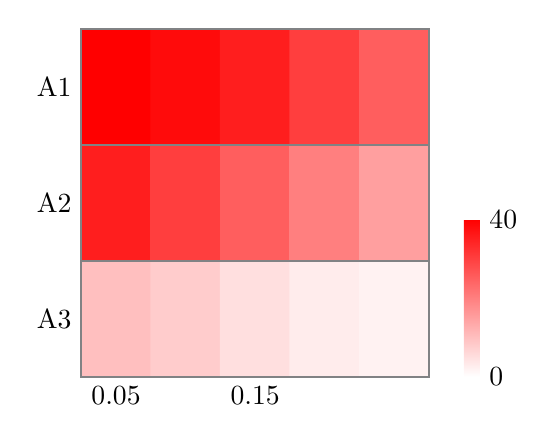
\begin{tikzpicture}
    \begin{axis}[
        width=6cm,
        height=6cm,
        yticklabels={A1, A2, A3},
        xticklabels={0.05, {}, 0.15},
        extra y ticks={0.5, 1.5},
        colorbar,
        colorbar style={
            width=2mm,
            height=2cm,
            ytick={0,40},
        },
        point meta min=0,
        point meta max=40,
        ]
        \addplot[
            matrix plot,
            mesh/cols=5,
            point meta=explicit,
        ] table [meta=C] {
            x y  C
            0 0  40
            1 0  38
            2 0  35
            3 0  30
            4 0  25
            0 1  35
            1 1  30
            2 1  25
            3 1  20
            4 1  15
            0 2  10
            1 2  8
            2 2  5
            3 2  3
            4 2  2
        };
    \end{axis}
\end{tikzpicture}

\end{document}
